\FloatBarrier  %
\section{Results on GPT-6 Luna}
\label{app:results}

We run three harnesses on GPT-6 Luna, a commercial model, at low, medium and high reasoning effort: prime-agent \citep{karten2026primeagent}, hermes-agent \citep{nous2026hermesagent} and openclaw \citep{openclaw2026}, each with its persistence on, as it ships (H), and with its persistence switched off (H\textsubscript{0}), beside the two floors and the program library. GPT-6 Luna's weights are closed, so this grid has no trained method, and it checks what prime-agent does on the open models against two other harnesses.

Figure~\ref{fig:plane-luna} draws the grid at high effort, with each harness also asked to store (H-A) and given the expert guidance (H-E, Appendix~\ref{app:ablations}), and Table~\ref{tab:tests-luna} gives the frozen tests at every effort. Figure~\ref{fig:luna-cost} sets each system's share learned on the stream against what its model calls cost. The records of every cell come with the paper (the reproducibility statement).

\paragraph{The two models.}
GLM-5.3 Flash and GPT-6 Luna are strong in different ways. On Artificial Analysis's Intelligence Index (v4.3.2), GLM-5.3 Flash scores 42 against 33 for GPT-6 Luna at high effort, with its widest margin on Terminal-Bench, 33 against 5\% \citep{artificialanalysis2026index}. At first sight on ARC the order reverses: from three demonstrations, GLM-5.3 Flash solves 26.8\% of the track's public tasks against 62.5 for GPT-6 Luna at high effort (Table~\ref{tab:heldout}). In the harness the two solve about as often. Once every task has been met, GLM-5.3 Flash in prime-agent solves \sbGlmHzeroSolved{}\% of instances with its notes wiped (Table~\ref{tab:solved}), and GPT-6 Luna at high effort \sbLunaHzeroSolvedMin{} to \sbLunaHzeroSolvedMax{}\% in its three harnesses.

\paragraph{The share learned.}
\label{sec:luna}

\begin{figure}[htbp]
\centering
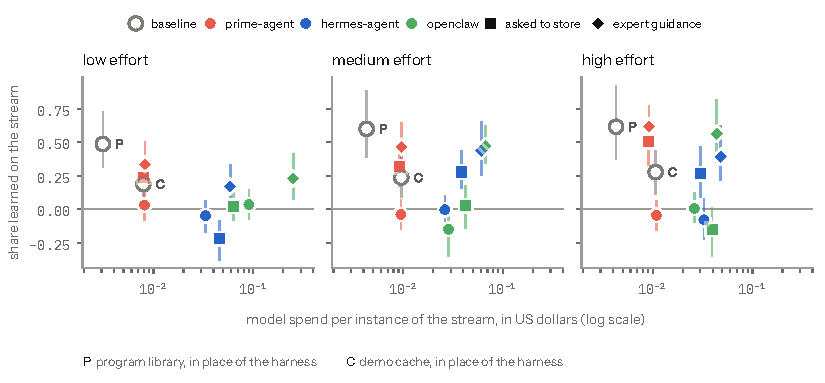
\includegraphics[width=\linewidth]{figures/luna-cost.pdf}
\caption{The share learned on the stream (Equation~\ref{eq:learned}, higher is better) of every GPT-6 Luna system that keeps something, with its 95\% interval, against what its model calls cost per instance of the stream (log scale), a panel per effort: each harness in its color, as it ships (circle), asked to store (square) and given the expert guidance (diamond), beside the program library (P) and the demo-cache floor (C). Each system is read against itself reset before every instance. The program library learns as much as any system for the least spend.}
\label{fig:luna-cost}
\end{figure}

On GPT-6 Luna, no harness as shipped saves a measurable share of the learnable budget at any reasoning effort (Figure~\ref{fig:luna-cost}). Against their own methods H\textsubscript{0}, the persistent methods lie between $-0.15$ and 0.04, and every 95\% interval includes zero, while the program library saves 0.49 [0.31, 0.73] of its learnable budget at low effort, 0.60 [0.38, 0.88] at medium and 0.62 [0.37, 0.93] at high, and the demo-cache floor, which only keeps the pairs it bought, saves 0.19 [0.10, 0.29], 0.24 [0.09, 0.40] and 0.28 [0.11, 0.44] of its own. The learnable budget of the model alone falls as the effort rises, from 50.8 points at low effort to 26.5 at high, because a stronger model pays less on every instance, returns included. A model that leaves little of it has outgrown the track (Section~\ref{sec:metrics}).

The state that each harness stored shows why the harnesses saved nothing (Appendix~\ref{app:persist}). Left to decide, none stored what answered a returning task. The three are built for lessons that transfer across unrelated work, none ties its store to the task id, and each breaks at a different step between an instance and its return. prime-agent kept nothing beyond a session in any of its three persistent cells, so the digest of its store that it shows the model was empty on every return. hermes-agent always shows the model what it stored, but it stores general advice on how to approach a task, with files named for a task only at low effort, where the re-exposures on which one came back cost more than the rest. openclaw seldom searches its history, and its consolidation never writes a memory, so no earlier correct answer came back on any re-exposure its replay log holds. Told what to keep, they keep it: with the expert guidance, the program library's procedure, added to their rules (method \mbox{H-E}, Appendix~\ref{app:ablations}), every harness saves a measurable share of its learnable budget at every effort, 0.17 to 0.62 against the same harness given the guidance and wiped (method \mbox{H-E\textsubscript{0}}), and prime-agent's matches the program library within noise at medium and high effort, and openclaw's at high. The harnesses on GPT-6 Luna therefore memorize when they are told what to keep, as GLM-5.3 Flash's harness does, while Qwen3.5-9B's, told the same, saved nothing measurable (Section~\ref{sec:results}).

\paragraph{The model and its presets.}
\label{sec:models}
We choose the models from the ARC Prize leaderboard at the time of submission. A preset (a model at one reasoning effort) qualifies when its verified semi-private zero-shot score lies between about 15 and 60\%, the band in which we expect a harness to have room to learn. One model family, GPT-6 Luna, covers the track from within the band at the lowest cost on the board, and we use its reasoning effort as the ability axis. We run low, medium and high effort on ARC-AGI-1, the last above the band. The board is measured on the evaluation set, but the ARC-AGI-1 stream serves easier, generated training instances. For this reason, we also check each preset against the stateless floor's first-exposure solve rate on the stream itself. On ARC-AGI-1, pooled with the side experiment's two orders, the stateless floor solved 33\% of its 75 first exposures at first answer at low effort, 61 at medium and 67 at high, against board scores of 37.7, 61.0 and 70.3\%. Low and medium effort leave room to learn. On every preset we run, the model alone leaves a learnable budget of 26.5 to 50.8 points. On ARC-AGI-1, every method runs at every effort, which lets us compare the harnesses on identical weights at each effort.

\paragraph{The charge these runs were played under.}
\label{sec:charge}
Every GPT-6 Luna cell, the side experiment's on the order among them, and its frozen tests, was played under rules that state the charge of Equation~\ref{eq:score} (Appendix~\ref{app:prompts}). The rules were first written for an earlier charge, under which an instance that ended unsolved cost the attempt cap, 8, plus its demonstrations. Under the current charge a learner that will fail anyway loses nothing by buying every demonstration before its last attempt, so the rules it reads can change its play. We therefore played GPT-6 Luna's cells again under the current rules rather than charge their records again, and no cell played under the earlier rules enters a number we report.

\paragraph{The frozen tests.}
After the stream, every system plays the two tests of Section~\ref{sec:tests} from its final state, and the reset plays them from an empty state, apart from it (Table~\ref{tab:tests-luna}). A system that keeps nothing between instances, a floor or a wiped method, reads half its plays against the other half, so its spread, $-0.06$ to 0.13 on the seen test and $-0.17$ to 0.07 on the held-out test, is the noise of playing a test. Judged with the other learners of its effort (Appendix~\ref{app:bench}), every method that kept a program per task saved more than chance on the seen test, as did the demo-cache floor and prime-agent asked to store, while the harnesses as shipped did not. On the held-out test, none of the 30 readings of the methods that keep something saved more than chance once each effort's eleven learners are judged together, and four cost more, three of them hermes-agent's. The tests detect memorization, and no positive held-out saving survives the correction.

\begin{table}[htbp]
\centering
\footnotesize\setlength{\tabcolsep}{3pt}
\begin{adjustbox}{max width=\linewidth}
\begin{tabular}{lr@{\hspace{0.4em}}lr@{\hspace{0.4em}}lr@{\hspace{0.4em}}lr@{\hspace{0.4em}}lr@{\hspace{0.4em}}lr@{\hspace{0.4em}}l}
\toprule
method & \multicolumn{6}{c}{share saved on the seen test} & \multicolumn{6}{c}{share saved on the held-out test} \\
\cmidrule(lr){2-7}\cmidrule(lr){8-13}
 GPT-6 Luna, effort & \multicolumn{2}{c}{low} & \multicolumn{2}{c}{medium} & \multicolumn{2}{c}{high} & \multicolumn{2}{c}{low} & \multicolumn{2}{c}{medium} & \multicolumn{2}{c}{high} \\
\midrule
\multicolumn{13}{l}{\emph{floors}} \\
stateless & 0.00 & {\scriptsize [-0.07, +0.06]} & +0.12 & {\scriptsize [+0.01, +0.24]} & -0.04 & {\scriptsize [-0.14, +0.05]} & +0.02 & {\scriptsize [-0.03, +0.07]} & -0.04 & {\scriptsize [-0.15, +0.08]} & -0.12 & {\scriptsize [-0.23, -0.02]} \\
demo-cache & +0.21 & {\scriptsize [+0.08, +0.36]} & +0.34 & {\scriptsize [+0.22, +0.48]} & +0.51 & {\scriptsize [+0.38, +0.67]} & +0.03 & {\scriptsize [0.00, +0.07]} & 0.00 & {\scriptsize [-0.07, +0.07]} & -0.01 & {\scriptsize [-0.10, +0.07]} \\
\midrule
\multicolumn{13}{l}{\emph{program library}} \\
PL\textsubscript{0} & +0.02 & {\scriptsize [-0.06, +0.09]} & -0.04 & {\scriptsize [-0.14, +0.05]} & +0.05 & {\scriptsize [-0.05, +0.13]} & +0.07 & {\scriptsize [-0.03, +0.15]} & +0.05 & {\scriptsize [-0.08, +0.16]} & -0.02 & {\scriptsize [-0.11, +0.05]} \\
PL & \textbf{+0.54} & {\scriptsize [+0.35, +0.78]} & \textbf{+0.77} & {\scriptsize [+0.54, +0.97]} & \textbf{+0.73} & {\scriptsize [+0.47, +0.98]} & -0.06 & {\scriptsize [-0.12, 0.00]} & -0.06 & {\scriptsize [-0.15, +0.04]} & -0.02 & {\scriptsize [-0.08, +0.05]} \\
\midrule
\multicolumn{13}{l}{\emph{hermes-agent}} \\
H\textsubscript{0} & +0.04 & {\scriptsize [-0.05, +0.14]} & +0.01 & {\scriptsize [-0.07, +0.09]} & +0.01 & {\scriptsize [-0.12, +0.12]} & 0.00 & {\scriptsize [-0.08, +0.08]} & -0.17 & {\scriptsize [-0.35, -0.03]} & -0.07 & {\scriptsize [-0.20, +0.06]} \\
H-E\textsubscript{0} & +0.03 & {\scriptsize [-0.08, +0.13]} & -0.03 & {\scriptsize [-0.12, +0.06]} & +0.03 & {\scriptsize [-0.09, +0.13]} & +0.03 & {\scriptsize [-0.06, +0.12]} & +0.02 & {\scriptsize [-0.10, +0.13]} & 0.00 & {\scriptsize [-0.16, +0.13]} \\
H & +0.03 & {\scriptsize [-0.09, +0.15]} & -0.07 & {\scriptsize [-0.22, +0.05]} & +0.03 & {\scriptsize [-0.05, +0.10]} & -0.02 & {\scriptsize [-0.09, +0.04]} & -0.21 & {\scriptsize [-0.32, -0.10]} & -0.01 & {\scriptsize [-0.09, +0.06]} \\
H-A & -0.04 & {\scriptsize [-0.22, +0.13]} & +0.18 & {\scriptsize [+0.05, +0.35]} & +0.18 & {\scriptsize [-0.01, +0.39]} & -0.25 & {\scriptsize [-0.34, -0.17]} & -0.09 & {\scriptsize [-0.18, 0.00]} & -0.01 & {\scriptsize [-0.11, +0.07]} \\
H-E & +0.30 & {\scriptsize [+0.14, +0.49]} & +0.52 & {\scriptsize [+0.36, +0.71]} & +0.62 & {\scriptsize [+0.45, +0.81]} & -0.09 & {\scriptsize [-0.16, -0.03]} & \textbf{+0.11} & {\scriptsize [+0.01, +0.19]} & \textbf{+0.13} & {\scriptsize [+0.04, +0.21]} \\
\midrule
\multicolumn{13}{l}{\emph{openclaw}} \\
H\textsubscript{0} & +0.01 & {\scriptsize [-0.08, +0.09]} & -0.06 & {\scriptsize [-0.15, +0.01]} & 0.00 & {\scriptsize [-0.10, +0.10]} & -0.04 & {\scriptsize [-0.12, +0.04]} & -0.11 & {\scriptsize [-0.27, +0.02]} & +0.02 & {\scriptsize [-0.11, +0.14]} \\
H-E\textsubscript{0} & +0.06 & {\scriptsize [-0.02, +0.14]} & +0.01 & {\scriptsize [-0.12, +0.13]} & 0.00 & {\scriptsize [-0.08, +0.08]} & -0.02 & {\scriptsize [-0.11, +0.07]} & -0.02 & {\scriptsize [-0.14, +0.08]} & +0.06 & {\scriptsize [-0.05, +0.15]} \\
H & -0.04 & {\scriptsize [-0.13, +0.03]} & +0.02 & {\scriptsize [-0.09, +0.12]} & -0.04 & {\scriptsize [-0.12, +0.03]} & +0.01 & {\scriptsize [-0.05, +0.07]} & -0.06 & {\scriptsize [-0.17, +0.04]} & -0.05 & {\scriptsize [-0.13, +0.03]} \\
H-A & -0.11 & {\scriptsize [-0.21, -0.02]} & +0.04 & {\scriptsize [-0.08, +0.18]} & +0.07 & {\scriptsize [-0.02, +0.17]} & -0.07 & {\scriptsize [-0.14, 0.00]} & 0.00 & {\scriptsize [-0.10, +0.10]} & -0.14 & {\scriptsize [-0.23, -0.04]} \\
H-E & +0.28 & {\scriptsize [+0.12, +0.48]} & +0.58 & {\scriptsize [+0.38, +0.78]} & +0.64 & {\scriptsize [+0.44, +0.82]} & -0.06 & {\scriptsize [-0.14, 0.00]} & +0.02 & {\scriptsize [-0.07, +0.11]} & -0.02 & {\scriptsize [-0.11, +0.06]} \\
\midrule
\multicolumn{13}{l}{\emph{prime-agent}} \\
H\textsubscript{0} & -0.05 & {\scriptsize [-0.17, +0.05]} & +0.02 & {\scriptsize [-0.11, +0.14]} & +0.02 & {\scriptsize [-0.14, +0.14]} & +0.03 & {\scriptsize [-0.07, +0.12]} & -0.05 & {\scriptsize [-0.22, +0.09]} & -0.08 & {\scriptsize [-0.21, +0.05]} \\
H-E\textsubscript{0} & -0.03 & {\scriptsize [-0.13, +0.06]} & +0.13 & {\scriptsize [0.00, +0.24]} & +0.07 & {\scriptsize [-0.01, +0.15]} & +0.04 & {\scriptsize [-0.04, +0.12]} & -0.01 & {\scriptsize [-0.15, +0.11]} & -0.05 & {\scriptsize [-0.23, +0.10]} \\
H & -0.02 & {\scriptsize [-0.09, +0.05]} & +0.06 & {\scriptsize [-0.03, +0.14]} & -0.05 & {\scriptsize [-0.17, +0.04]} & 0.00 & {\scriptsize [-0.05, +0.06]} & -0.03 & {\scriptsize [-0.15, +0.07]} & +0.06 & {\scriptsize [-0.05, +0.14]} \\
H-A & +0.19 & {\scriptsize [+0.08, +0.35]} & +0.37 & {\scriptsize [+0.27, +0.49]} & +0.42 & {\scriptsize [+0.29, +0.55]} & +0.01 & {\scriptsize [-0.05, +0.07]} & +0.05 & {\scriptsize [-0.06, +0.15]} & +0.12 & {\scriptsize [+0.03, +0.21]} \\
H-E & +0.35 & {\scriptsize [+0.17, +0.58]} & +0.57 & {\scriptsize [+0.34, +0.80]} & +0.72 & {\scriptsize [+0.63, +0.82]} & +0.02 & {\scriptsize [-0.05, +0.08]} & 0.00 & {\scriptsize [-0.10, +0.08]} & +0.05 & {\scriptsize [-0.03, +0.12]} \\
\bottomrule
\end{tabular}

\end{adjustbox}
\caption{GPT-6 Luna's frozen tests: the share of the reset's spend on each test that a system no longer pays, against itself reset (Equation~\ref{eq:transfer}, higher is better), with its 95\% interval over task resamples in small type. A harness is read against its method H\textsubscript{0}, and \mbox{H-E} against \mbox{H-E\textsubscript{0}}; the demo-cache floor against the stateless floor, and the program library against PL\textsubscript{0}. A floor or a wiped method reads half its plays against the other half, so these methods show the noise of playing a test. Bold marks each column's best among the values whose 95\% interval lies above zero.}
\label{tab:tests-luna}
\end{table}
